\documentclass[10pt,UTF8,twocolumn,a4paper]{ctexart}
\usepackage{amsmath,amsthm,amsfonts,amssymb,bm}
\usepackage{graphicx, geometry}
\usepackage{multicol}
\usepackage{setspace}
\usepackage{unicode-math}
\usepackage{anyfontsize}
\usepackage{fontspec}
\usepackage{extarrows}
\usepackage{array}
\usepackage{float}
% \setlength\columnsep{10pt}
\xeCJKsetup{CJKmath=true}
\setmainfont{FandolHei-Regular}       % XITS 是 Times Roman 的开源复刻版本
\setmathfont{XITS Math}
\linespread{0.1}
\geometry{a4paper, left=0.5cm, right=0.5cm, top=0.2cm, bottom=0.5cm}

\begin{document}
\small
\noindent

    \hrule
    ~\\
    \symbol{"2460} 常见级数展开和麦克劳林公式:
    $$
    \begin{array}{@{}c@{}c@{}c@{}c@{\thinspace}l@{}l@{}l}
        e^x    &=&\sum_{n=0}^{\infty}\frac{x^n}{n!}
               &=&1+x+\frac{x^2}{2}+o(x^2)                      &x&\in(-\infty,+\infty)\\[5pt]
        \ln(1+x) &=&\sum_{n=1}^\infty\frac{(-1)^{n-1}}{n}x^{n}
                 &=&x-\frac{x^2}{2}+\frac{x^3}{3}+o(x^3)        &x&\in(-1, 1]\\[5pt]
        \ln(1-x) &=&-\sum_{n=1}^\infty\frac{x^{n}}{n}
                 &=&-(x+\frac{x^2}{2}+\frac{x^3}{3}+o(x^3))     &x&\in[-1, 1)\\[5pt]
        \frac{1}{1-x} &=&\sum_{n=0}^\infty{x^n}
                      &=& 1+x+x^2+x^3+o(x^3)                    &x&\in(-1, 1)\\[5pt]
        \frac{1}{1+x} &=&\sum_{n=0}^\infty{(-1)^nx^n}
                      &=&1-x+x^2-x^3+o(x^3)                     &x&\in(-1, 1)\\[5pt]
        (1+x)^\alpha  &=&1+\sum_{n=1}^{\infty}\frac{\prod_{i=0}^{n-1}(\alpha-i)}{n!}x^n
                      &=&1+\alpha x+\frac{\alpha(\alpha-1)}{2!}x^2+o(x^2)   &x&\in\left(-1, 1\right)\\[5pt]
        (1+x)^{\frac{1}{x}} &=&可由(2)推得
                            &=&e-\frac{e}{2}x+\frac{11e}{24}x^2-\frac{7e}{16}x^3+o(x^3)\\[6pt]
        \sin x  &=&\sum_{n=0}^{\infty}\frac{(-1)^n}{(2n+1)!}x^{2n+1}
                &=&x-\frac{x^3}{6}+\frac{x^5}{120}+o(x^5)       &x&\in(-\infty,+\infty)\\[6pt]
        \cos x  &=&\sum_{n=0}^{\infty}\frac{(-1)^n}{(2n)!}x^{2n}
                &=&1-\frac{x^2}{2}+\frac{x^4}{24}+o(x^4)        &x&\in(-\infty,+\infty)\\[5pt]
        \tan x  &=&\sum_{n=1}^{\infty}\frac{(4^n-1)\zeta(2n)}{\pi^{2n}}x^{2n-1}
                &=&x+\frac{1}{3}x^3+\frac{2}{15}x^5+o(x^5)      &x&\in\left(-\frac{\pi}{2},\frac{\pi}{2}\right)\\[5pt]
        \arcsin x   &=&\sum_{n=0}^{\infty}\frac{C_{2n}^n}{4^n(2n+1)}x^{2n+1}
                    &=&x+\frac{1}{6}x^3+\frac{3}{40}x^5+o(x^5)  &x&\in\left(-1, 1\right)\\[6pt]
        \arccos x   &=&\frac{2}{\pi} - \arcsin x
                    &=&\frac{2}{\pi}-x-\frac{1}{6}x^3-\frac{3}{40}x^5+o(x^5) &x&\in\left(-1, 1\right)\\[5pt]
        \arctan x   &=&\sum_{n=0}^{\infty}\frac{(-1)^n}{2n+1}x^{2n+1}
                    &=&x-\frac{1}{3}x^3+\frac{1}{5}x^5+o(x^5)   &x&\in\left[-1, 1\right] \\[5pt]
    \end{array}
    $$

    $$
    \begin{array}{l}
        f(x)\sim\frac{a_0}{2}+\sum_{n=1}^\infty(a_n\cos nx + b_n\sin nx) \quad
        \begin{cases}
            a_n = \frac{1}{l}\int_{-l}^{l}f(x)\cos\frac{n\pi x}{l} \mathrm{d}x \\[10pt]
            b_n = \frac{1}{l}\int_{-l}^{l}f(x)\sin\frac{n\pi x}{l} \mathrm{d}x
        \end{cases}
    \end{array}\\[5pt]
    $$
    ~\\
    
    \hrule
    ~\\
    \symbol{"2461} 常用积分:

    \begin{multicols}{2}
    \scriptsize
    \begin{flushleft}
    $
        \begin{array}{@{}c@{\thinspace}c@{\thinspace}ll}
            \int x^\alpha\mathrm{d}x    &=& \frac{1}{\alpha+1}x^{\alpha+1}+C, \quad (a\neq-1)   \\[5pt]
            \int a^x\mathrm{d}x         &=& \frac{a^x}{\ln a} + C,            \quad (a>0,a\neq1)\\[5pt]
            \int e^x\mathrm{d}x         &=& e^x +C       \\[5pt]
            \int \sin x\mathrm{d}x      &=& -\cos x +C   \\[5pt]
            \int \cos x\mathrm{d}x      &=& \sin x +C    \\[5pt]
            \int \tan x\mathrm{d}x      &=& -\ln|\cos x|+ C \\[5pt]
            \int \cot x\mathrm{d}x      &=& \ln|\sin x| + C  \\[5pt]
            \int \sec x\mathrm{d}x      &=& \ln|\sec x+\tan x|+C \\[5pt]
            \int \csc x\mathrm{d}x      &=& \ln|\csc x-\cot x|+C \\[5pt]
            \int \sec^2x\mathrm{d}x     &=& \tan x +C            \\[5pt]
            \int \csc^2x\mathrm{d}x     &=& -\cot x +C           \\[5pt]
        \end{array}
    $
    $
    \begin{array}{@{}c@{\thinspace}c@{\thinspace}ll}
        \int \frac{1}{x}\mathrm{d}x &=& \ln |x| + C  \\[5pt]
        \int \frac{1}{a^2+x^2}\mathrm{d}x           &=& \frac{1}{a}\arctan\frac{x}{a}                   \\[5pt]
        \int \frac{1}{a^2-x^2}\mathrm{d}x           &=& \frac{1}{2a}\ln \left|\frac{a+x}{a-x}\right| + C\\[5pt]
        \int \frac{1}{\sqrt{a^2+x^2}}\mathrm{d}x    &=& \arcsin\frac{x}{a} + C                          \\[5pt]
        \int \frac{1}{\sqrt{x^2\pm a^2}}\mathrm{d}x &=& \ln\left|x+\sqrt{x^2\pm a^2}\right| + C         \\[7pt]
        \int\! \sqrt{a^2\!-\!x^2}dx       &=& \frac{x}{2}\sqrt{a^2\!-\!x^2}\!+\!\frac{a^2}{2}\arcsin\frac{x}{a}+C     \\[5pt]
        \int\! \sqrt{x^2\!-\!a^2}dx       &=& \frac{x}{2}\sqrt{x^2\!-\!a^2}\!-\!\frac{a^2}{2}\!\ln\!|x\!+\!\sqrt{x^2\!-\!a^2}|\!+\!C     \\[5pt]
        \int\! \sqrt{x^2\!+\!a^2}dx       &=& \frac{x}{2}\sqrt{x^2\!+\!a^2}\!+\!\frac{a^2}{2}\!\ln(x\!+\!\sqrt{x^2\!+\!a^2})\!+\!C     \\[5pt]
    \end{array}
    $   
    \end{flushleft}
    
    \end{multicols}

    \hrule
    ~\\
    \symbol{"2462} 积分公式:
    $$
    \begin{cases}
        \int R\left(x,\sqrt{a^2-x^2}\right)\mathbf{d}x  \xlongequal{x=a\sin t} \int R\left(a\sin t, a\cos t\right)a\cos t  \mathbf{d}t \\[8pt]
        \int R\left(x,\sqrt{x^2+a^2}\right)\mathbf{d}x  \xlongequal{x=a\tan t} \int R\left(a\tan t, a\sec t\right)a\sec^2t \mathbf{d}t \\[8pt]
        \int R\left(x,\sqrt{x^2-a^2}\right)\mathbf{d}x  \xlongequal{x=a\sec t} \int R\left(a\sec t, a\tan t\right)a\sec t\tan t \mathbf{d}t \\[8pt]
        \int R\left(x, \sqrt[n]{ax+b}, \sqrt[m]{ax+b}\right)\mathbf{d}x  \xlongequal{\sqrt[mn]{ax+b}=t}  \int R\left(\frac{t^{mn}-b}{a}, t^m, t^n\right)\frac{mn}{a}t^{mn-1}\mathbf{d}t \\[8pt]
        \int R\left(x, \sqrt{\frac{ax+b}{cx+d}}\right)\mathbf{d}x  \xlongequal{\sqrt{\frac{ax+b}{cx+d}}=t}  \int R\left(\frac{dt^2-b}{a-ct^2}, t\right)\frac{2(ad-bc)t}{(a-ct^2)^2}\mathbf{d}t \quad (ad-bc\neq0)\\[8pt]
        \int R\left(\sin x, \cos x\right)\mathbf{d}x  \xlongequal[\tan\frac{x}{2}=t]{\sin x=\frac{2t}{1+t^2}, \cos x=\frac{1-t^2}{1+t^2}}  \int R\left(\frac{2t}{1+t^2}, \frac{1-t^2}{1+t^2}\right)\frac{2}{1+t^2}\mathbf{d}t
    \end{cases}
    $$

    $$
    \begin{array}{l}
        \int_0^{\frac{\pi}{2}}\sin^nx \mathrm{d}x = \int_0^{\frac{\pi}{2}}\cos^nx \mathrm{d}x 
            = \begin{cases}
                \frac{n-1}{n}\cdot\frac{n-3}{n-2}\cdots\frac{1}{2}\cdot\frac{\pi}{2}, &(n>0,n为偶) \\[8pt]
                \frac{n-1}{n}\cdot\frac{n-3}{n-2}\cdots\frac{2}{3}\cdot1,             &(n>1,n为奇)
                \end{cases}
    \end{array}\\[5pt]
    $$
    $$
    \begin{array}{l}
    \int_0^\pi\sin^nx \mathrm{d}x = 2\cdot\int_0^{\frac{\pi}{2}}\sin^nx \mathrm{d}x, (n>0) \\[8pt]
    \int_0^\pi\cos^nx \mathrm{d}x = 
        \begin{cases}
            2\cdot\int_0^{\frac{\pi}{2}}\cos^nx \mathrm{d}x, & (n>0,n为偶) \\[8pt]
            0,                                               & (n>0,n为奇)
        \end{cases}
    \end{array}\\[5pt]
    $$
    $$
    \begin{array}{l}
        \int_0^{2\pi}\sin^nx \mathrm{d}x = \int_0^{2\pi}\cos^nx \mathrm{d}x 
            = \begin{cases}
                4\cdot\frac{n-1}{n}\cdot\frac{n-3}{n-2}\cdots\frac{1}{2}\cdot\frac{\pi}{2}, &(n>0,n为偶) \\[8pt]
                0,             &(n>0,n为奇)
                \end{cases}
    \end{array}\\[5pt]
    $$

    $$
    \begin{array}{c}
    % \begin{array}{@{}c@{\thinspace}c@{\thinspace}l}
        \int x^ne^{-x}\mathrm{d}x = -e^{-x}\sum_{i=0}^n{(x^n)^{(i)}} + C \quad
        \int x^ne^{x}\mathrm{d}x =  e^{x}\sum_{i=0}^n{(-1)^i (x^n)^{(i)}} + C \\[5pt]
        \int_0^{+\infty}x^ne^{-x}\mathrm{d}x =\ n! = \Gamma(n+1)              \\[5pt]
        \int_{-\infty}^{+\infty} e^{-x^2}\mathrm{d}x = \sqrt{\pi}
    \end{array}
    $$\\[5pt]


    \hrule
    ~\\
    \symbol{"2463} 微分导数相关:
    $$
        \begin{array}{l}
            (uv)^{(n)} = \sum_{i=0}^n \mathrm{C}_n^iu^{(n-i)}v^{(i)}
        \end{array}\\[5pt]
    $$
    

    \begin{multicols}{2}
        \scriptsize
        \multicolsep = 5pt
        \columnsep = 1pt
        
        $
            \begin{array}{@{}c@{\thinspace}c@{\thinspace}l}
                (e^{ax})^{(n)} &=& a^{n}e^{ax} \\[8pt]
                (\sin ax)^{(n)} &=& a^n\sin\left(\frac{n\pi}{2}+ax\right) \\[8pt]
                (\cos ax)^{(n)} &=& a^n\cos\left(\frac{n\pi}{2}+ax\right)
            \end{array}
        $

        $
            \begin{array}{@{}c@{\thinspace}c@{\thinspace}l}
                (\ln(1+x))^{(n)} &=& \frac{(-1)^{n-1}(n-1)!}{(1+x)^n}\\[8pt]
                ((1+x)^\alpha)^{(n)} &=& \prod_{i=0}^{n-1}(a-i)(1+x)^{\alpha-n}\\[8pt]
                ((1+x)^n)^{(n)} &=& n! \quad ((1+x)^n)^{(n+j)} = 0
            \end{array}
        $
    \end{multicols}

    \begin{center}
    $
        R=\frac{|y''|}{(1+y'^2)^{3/2}} \quad 曲率k=\frac{1}{R} \quad 曲率中心(\alpha, \beta)=\left(x-\frac{y'(1+y'^2)}{y''}, y+\frac{1+y'^2}{y''}\right)
    $\\[5pt]
    \end{center}
    


    \hrule
    ~\\
    \symbol{"2464} 解析几何:
    $$ d_{点面}=\frac{|Ax_0+By_0+Cz_0+D|}{\sqrt{A^2+B^2+C^2}} \qquad  d_{线线}=\frac{\left|(\mathbb{s}_1\mathbb{s}_2\vec{AB})\right|}{|\mathbb{s}_1\times\mathbb{s}_1|} \\[5pt]$$
    $$ d_{点线}=\frac{|\{x_1-x_0, y_1-y_0, z_1-z_0\}\times\{l,m,n\}|}{\sqrt{l^2+m^2+n^2}}$$
    
    $$ 
    \begin{array}{l}
    直线\begin{cases}
        A_1x+B_1y+C_1z+D_1 = 0\\
        A_2x+B_2y+C_2z+D_2 = 0\\
        \end{cases}\\
    的平面束: \lambda (A_1x+B_1y+C_1z+D_1)+\mu (A_2x+B_2y+C_2z+D_2) = 0 \\
    或: (A_1x+B_1y+C_1z+D_1)+k (A_2x+B_2y+C_2z+D_2) = 0 \quad \left(k=\frac{\mu}{\lambda}\right)
    \end{array}
    $$

    \begin{table}[H]
    \centering
    \begin{tabular}{m{2.5cm} m{1.5cm} m{2.5cm} m{1.5cm}}
        $\frac{x^2}{a^2}+\frac{y^2}{b^2}+\frac{z^2}{c^2} = 1$    &  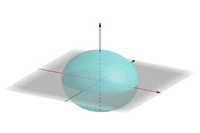
\includegraphics[width=40pt]{image/Ellipsoidal_Surface.png}   &  $\frac{x^2}{a^2}+\frac{y^2}{b^2}-2pz = 0$   &  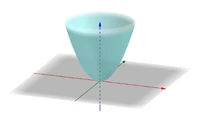
\includegraphics[width=40pt]{image/Elliptic_paraboloid.png}\\
        $\frac{x^2}{a^2}+\frac{y^2}{b^2}-\frac{z^2}{c^2} = 1$    &  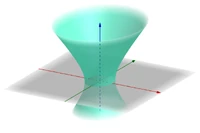
\includegraphics[width=40pt]{image/Univalent_hyperboloid.png} &  $\frac{x^2}{a^2}-\frac{y^2}{b^2}-2pz = 0$   &  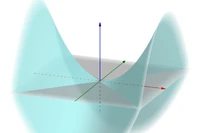
\includegraphics[width=40pt]{image/Hyperbolic_paraboloid.png}\\
        $\frac{x^2}{a^2}+\frac{y^2}{b^2}-\frac{z^2}{c^2} = -1$   &  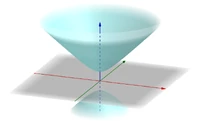
\includegraphics[width=40pt]{image/Bilobal_hyperboloid.png}   &  $\frac{x^2}{a^2}+\frac{y^2}{b^2}-\frac{z^2}{c^2} = 0$    &  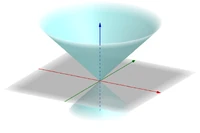
\includegraphics[width=40pt]{image/Quadric_Cone.png}\\
    \end{tabular}
    \end{table}

    \hrule
    ~\\
    \symbol{"2465} 多元微积分:
    $$  
    \begin{array}{l}
        \thinspace\thinspace f_{xx}''(x_0, y_0)=A, f_{xy}''(x_0, y_0)=B, f_{yy}''(x_0, y_0)=C\\
        \begin{cases}
            AC-B^2>0  & A>0极小值,A<0极大值  \\
            AC-B^2<0  & 非极值 \\
            AC-B^2=0  & 无法判断
        \end{cases}
    \end{array}
    $$\\[5pt]
    

    \hrule
    ~\\
    \symbol{"2466} 常微分方程:
    $$
    \begin{array}{l}
        \boxed{y'=f(x)g(y)} \;\,   同除g(y)积分          \\[5.5pt]
        \boxed{y'+p(x)y=q(x)} \,   同乘e^{\int p(x)dx}积得y=e^{-\int p(x)dx}\left[C+\int q(x)e^{\int p(x)dx}dx\right]       \\[3pt]
        \boxed{P(x,y)dx+Q(x,y)dy=0}  \; 若\frac{\partial Q}{\partial x}=\frac{\partial P}{\partial y},求u(x,y)=C使du=Pdx+Qdy\\[5pt]
        \\[5pt]

        \boxed{y'=f(\frac{y}{x})}  \; 令u=\frac{y}{x},u'=\frac{y'x-y}{x^2}=\frac{y'-u}{x},代得xu'+u=f(u)(可分) \\[10pt]
        \boxed{y'=f(ax+by+c)} \; 令u=ax+by+c,u'=a+by'=a+bf(u)(可分)     \\[5.5pt]
        \boxed{y'=f(\frac{a_1x+b_1y+c_1}{a_2x+b_2y+c_2})} \; 令x=X+h,y=Y+k消去c_1c_2化为齐次                \\[12.5pt]
        \boxed{y' + p(x)y = q(x)y^\alpha, (\alpha\neq 0,1)} \; 令u=y^{1-\alpha},u'=(1-\alpha)y^{-\alpha}y',代得一阶         \\[5.5pt]
        \boxed{y'=\frac{h(y)}{p(y)x+q(y)}} \; 以y为自变量,得\frac{dx}{dy}=\frac{p(y)}{h(y)}x+\frac{q(y)}{h(y)} (一阶)            \\[12pt]
        \boxed{y'=\frac{h(y)}{p(y)x+q(y)x^\alpha}, (\alpha\neq 0,1)} \; 以y为自变量,得\frac{dx}{dy}=\frac{p(y)}{h(y)}x+\frac{q(y)}{h(y)}x^\alpha (伯)\\[5pt]
        \\[8pt]

        \boxed{y^{(n)}=f(x)} \;  n次积分,结果有n个任意常数                           \\[5.5pt]
        \boxed{y''=f(x,y')}  \;  令u=y',代得u'=f(x,u)(一阶),解得u后积分得y           \\[5.5pt]
        \boxed{y''=f(y,y')}  \;  令u=y',y''=\frac{du}{dx}=\frac{du}{dy}\frac{du}{dx}=u\frac{du}{dy},代得u\frac{u}{y}=f(y,u)    \\[5.5pt]
        \\[8pt]

        \boxed{y''+p(x)y'+q(x)y=f(x)及高阶线性微分方程} \; 解性质\&通解结构           \\[5pt]
        \\[8pt]

        \boxed{y''+py'+qy=0} \;  解\lambda^2+p\lambda+q=0,根的3种情对应3种通解    \\[5.5pt]
        \boxed{y^{(n)}+p_1y^{(n-1)}+\cdots + p_n y=0}  \;  解\lambda^n+p_1\lambda^{n-1}+\cdots+p_n=0,k重根3种情况    \\[5pt]
        \\[8pt]

        \boxed{y''+py'+qy=f(x)}
            \begin{cases}
                =P_n(x) \;\qquad 特解y^*=x^kH_n(x)                                                  \\[5pt]
                =P_n(x)e^{\alpha x} \quad 特解y^*=x^kH_n(x)e^{\alpha x}                             \\[5pt]
                =e^{\alpha x}\left[P_n(x)sin\beta x+Q_m(x)cos\beta x\right] \;                     \\[5pt]
                \quad 特解y^*=x^ke^{\alpha x}\left[R_l(x)sin\beta x+S_l(x)cos\beta x\right]        \\
                \qquad\qquad\qquad\qquad\qquad\qquad\qquad\quad _{l=max\{n,m\}}                   \\[10pt]
                (k为\alpha 或\alpha\pm i\beta 在特征方程中根重数)
            \end{cases}\\[37pt]
        \boxed{x^2y''+pxy'+qy=f(x)} \;  令u=\pm e^t,\frac{dy}{dx}=\frac{dy}{dt}\frac{1}{x},\frac{d^2y}{dx^2}=\left(\frac{d^2y}{dx^2}-\frac{dy}{dx}\right)\frac{1}{x^2}
    \end{array}
    $$
    \\[10pt]


    \hrule
    ~\\
    \symbol{"2467} 极限相关:
    $$
    \lim\limits_{f(x)\to\infty}(1+\frac{1}{f(x)})^{f(x)}=e \qquad  \lim\limits_{f(x)\to0}(1+f(x))^{\frac{1}{f(x)}}=e
    $$\\[10pt]  

    \newpage
    \hrule
    ~\\
    \symbol{"2468} 初等数学:
    $$
    \begin{array}{l}
    \cdot\; \underline{\textbf{三角函数}}\\[5pt]
    \sin(a+b)=\sin a\cos b+\cos a\sin b \quad \cos(a+b)=\cos a\cos b-\sin a\sin b \\[5pt]
    \tan(a+b)=\frac{\tan a+\tan b}{1-\tan a\tan b}  \qquad\qquad\quad  \alpha\sin a+\beta\cos a =\sqrt{\alpha^2+\beta^2}\sin(a+\varphi) \\[8pt]

    \cdot\;  \underline{\textbf{因式分解}}\\[5pt]
    (a+b)^3=a^3+3a^2b+3ab^2+b^3  \qquad  (a-b)^3=a^3-3a^2b+3ab^2-b^3               \\[5pt]
    a^3-b^3=(a-b)(a^2+ab+b^2)  \qquad\;\;\,  a^n-b^n=(a-b)(\sum_{i=0}^{n-1}a^{n-1-i}b^i)  \\[5pt]
    求根:x=\frac{-b\pm\sqrt{b^2-4ac}}{2a}  \qquad  韦达定理: x_1+x_2=-\frac{b}{a},x_1x_2=\frac{c}{a}  \\[8pt]

    \cdot\; \underline{\textbf{不等式}}\\[5pt]
    \boxed{||a|-|b||\leq |a\pm b|\leq |a|+|b|}  \qquad  \frac{2}{a^{-1}+b^{-1}}\leq\sqrt{ab}\leq\frac{a+b}{2}\leq\sqrt{\frac{a^2+b^2}{2}}_{(a,b>0)}  \\[5pt]
    ab\leq\left({\frac{a+b}{2}}\right)^2\leq\frac{a^2+b^2}{2}_{(a,b>0)} \quad \frac{(a+b)^2}{2}\leq a^2+b^2_{(a,b>0)}  \quad 2ab\leq a^2+b^2_{(a,b\in R)} \\[12pt]
    \boxed{\frac{n}{\sum_{i=1}^n a_i^{-1}}\leq\sqrt[n]{\prod_{i=1}^n a_i}\leq\frac{\sum_{i=1}^n a_i}{n}\leq\sqrt{\frac{\sum_{i=1}^na_i^2}{n}}_{(a_i>0)}}  \\[8pt]
    \boxed{\sqrt[\alpha]{\frac{\sum_{i=1}^na_i^\alpha}{n}}\geq\sqrt[\beta]{\frac{\sum_{i=1}^na_i^\beta}{n}}_{(\alpha>\beta,a_i>0)}}  \qquad a^3+b^3+c^3\geq 3abc_{(a,b,c>0)}\\[8pt]
    \boxed{(a_1^2+a_2^2+\cdots+a_n^2)(b_1^2+b_2^2+\cdots+b_n^2)\geq(a_1b_1+a_2b_2+\cdots+a_nb_n)^2_{(a_i,b_i\in R)}}  \\[8pt]
    (a_1^2+a_2^2+\cdots+a_n^2)\geq\frac{1}{n}(a_1+a_2+\cdots+a_n)^2 \quad\;\; a^2+b^2+c^2\geq ab+bc+ca           \\[8pt]
    ab>0\Rightarrow\frac{a}{b}+\frac{b}{a}\geq 2 \quad  ab<0\Rightarrow\frac{a}{b}+\frac{b}{a}\leq -2 \quad \boxed{\frac{b}{a}<\frac{b+m}{a+m}<1_{(a>b>0,m>0)}}  \\[12pt]
    \sin x<x<\tan x_{(0<x<\frac{\pi}{2})} \quad \sin x<x_{(x>0)} \quad \arcsin x\geq x\arctan x_{(a\leq x\leq 1)} \\[8pt]
    e^{f(x)}\geq f(x)+1,e^{f(x)}\geq ef(x) \quad \ln x\leq x-1_{(x>0)}  \quad  \frac{x}{1+x}\leq\ln(1+x)\leq x_{(x\geq 0)}\\[8pt]

    \cdot\; \underline{\textbf{数列}}\\[5pt]
    a_n=a_1+(n-1)d \Rightarrow S_n=\frac{n}{2}(a_1+a_n)=na_1+\frac{1}{2}n(n-1)d          \\[5pt]
    a_n=a_1q^{n-1}(q\neq 1) \Rightarrow S_n=\frac{a_1(1-q^n)}{1-q}=\frac{a_1-a_nq}{1-q}  \\[5pt]
    \sum_{k=1}^nk=\frac{n(n+1)}{2} \qquad  \sum_{k=1}^nk^2=\frac{n(n+1)(2n+1)}{6}
    \end{array}
    $$\\[10pt]  


    \hrule
    ~\\
    \symbol{"2469} 放缩和不等式:
    $$
        \begin{array}{l}
            (uv)^{(n)} = \sum_{i=0}^n \mathrm{C}_n^iu^{(n-i)}v^{(i)}
        \end{array}
    $$\\[10pt]  

    \newpage

    \hrule
    ~\\
    \symbol{"2460} 行列式
    \\[10pt]


    \hrule
    ~\\
    \symbol{"2461} 矩阵
    \\[10pt]


    \hrule
    ~\\
    \symbol{"2462} 向量
    \\[10pt]
    

    \hrule
    ~\\
    \symbol{"2463} 线性方程组
    \\[10pt]

    \hrule
    ~\\
    \symbol{"2464} 秩
    \\[10pt]


    \hrule
    ~\\
    \symbol{"2465} 等价相似合同
    \\[10pt]
    
    \newpage

    \hrule
    ~\\
    \symbol{"2460} 事件和概率运算:
    $$
    \begin{array}{ll}
        A\cup B=B\cup A & A\cap B = B\cap A \\[5pt]
        A\cup (B\cup C) = (A\cup B)\cup C & A\cap (B\cap C) = (A\cap B)\cap C \\[5pt]
        A\cup (B\cap C) = (A\cup B)\cap (A\cup C) &  A\cap (B\cup C) = (A\cap B)\cup (A\cap C) \\[5pt]
        \overline{\bigcup\limits_{i=1}^{n}A_i}=\bigcap\limits_{i=1}^n\overline{A_i}\quad \overline{\bigcap\limits_{i=1}^{n}A_i}=\bigcup\limits_{i=1}^n\overline{A_i} & \overline{A-B}=\overline{A}\cup B \\
    \end{array}\\[5pt]
    $$
    $$
    \begin{array}{l}
        P(A\cup B) = P(A) + P(B) - P(AB) \\[3pt]
        P(A\cup B\cup C) = P(A) + P(B) + P(C)
        \\ \qquad\qquad\qquad\qquad\quad\; - P(AB) -P(BC) -P(AC) + P(ABC) \\[8pt]

        P(A-B) = P(A) - P(AB) \\[7pt]

        P(A) > 0 时, P(AB)=P(A)P(B|A) \\[2pt]
        P(A_1\cdots A_{n-1}) > 0 时, P(A_1\cdots A_{n})=P(A_1)P(A_2|A_1)\cdots P(A_n|A_1\cdots A_{n-1}) \\[8pt]

        \bigcup_{i=1}^nB_i=\Omega, B_iB_j=\emptyset(i\neq j),P(B_k)>0时: \\
        P(A) = \sum_{i=1}^nP(B_i)P(A|B_i) \\[8pt]

        \bigcup_{i=1}^nB_i=\Omega, B_iB_j=\emptyset(i\neq j),P(A)>0,P(B_k)>0时: \\
        P(B_j|A) = \frac{P(B_j)P(A|B_j)}{\sum_{i=1}^nP(B_i)P(A|B_i)} \\[12pt]
    \end{array}
    $$
    
    \hrule
    ~\\
    \symbol{"2461} 分布和性质:
    $$
    \begin{array}{l}
        \boxed{X\sim B(n,p)\quad P\left\{X=k\right\}=C_n^kp^kq^{n-k}}\\[8pt]
        \begin{array}{l}
            \cdot\; E(X)=np   \quad   D(X)=np(1-p) \\[5pt]
            \cdot\; p_n与n有关,若\lim\limits_{n\to\infty}np_n=\lambda, 则\lim\limits_{n\to\infty}C_n^kp^k_n(1-p_n)^{n-k}=\frac{\lambda^k}{k!}e^{-\lambda} \\[2pt]
            \cdot\; n\ge100,p\le0.1,C_n^kp^k(1-p)^{n-k}\approx\frac{(np)^k}{k!}e^{-np} \\[2pt]
        \end{array}\\[20pt]

        \boxed{X\sim G(p)\quad P\left\{X=k\right\}=pq^{k-1}}\\[8pt]
        \begin{array}{l}
            \cdot\; E(X)=\frac{1}{p}   \quad   D(X)=\frac{1-p}{p^2} \\[2pt]
        \end{array}\\[10pt]

        \boxed{X\sim H(n, N, M)\quad P\left\{X=k\right\}=\frac{C_M^kC_{N-M}^{n-k}}{C_N^n} }\\[20pt]

        \boxed{X\sim P(\lambda)\quad  P\left\{X=k\right\}=\frac{\lambda^k}{k!}e^{-\lambda}}\\[12pt]
        \begin{array}{l}
            \cdot\; E(X)=\lambda    \quad    D(X)=\lambda \\[2pt]
            \cdot\; X_1\sim P(\lambda_1),X_2\sim P(\lambda_2), X_1X_2独立 \Rightarrow X_1+X_2=P(\lambda_1+\lambda_2)  \\[2pt]
        \end{array}\\[15pt]

        \boxed{X\sim U(a,b)\quad  f(x)=\begin{cases}
                                            \frac{1}{b-a},\quad x\leq x\leq b \\
                                            0,\quad 其他 
                                        \end{cases}
        }\\[13pt]      
        \begin{array}{l}
            \cdot\; E(X)=\frac{a+b}{2}\quad  D(X)=\frac{(b-a)^2}{12}
        \end{array}\\[15pt]

        \boxed{X\sim E(\lambda)\quad  f(x)=\begin{cases}
                                                \lambda e^{-\lambda x},\quad x>0 \\
                                                0,\quad x\leq0 
                                            \end{cases}
        }\\[12pt]
        \begin{array}{l}
            \cdot\; E(X)=\frac{1}{\lambda}\quad   D(X)=\frac{1}{\lambda^2} \\[6pt]
            \cdot\; P\left\{X>t+s|X>s\right\}=\frac{e^{-\lambda(t+s)}}{e^{-\lambda s}}=e^{-\lambda t}=P\left\{X>t\right\},\quad (t,s>0)\\[2pt]
        \end{array}\\[15pt]

        \boxed{X\sim N(\mu, \sigma^2)\quad  f(x)=\frac{1}{\sqrt{2\pi}\sigma}e^{-\frac{(x-\mu)^2}{2\sigma^2}} }\\[16pt]
        \begin{array}{l}
            \cdot\; E(X)=\mu\quad        D(X)=\sigma^2        \\[2pt]
        \end{array}\\[10pt]

        \boxed{(X,Y)\sim N_{(\mu_1, \mu_2;\sigma_1^2,\sigma_2^2;\rho)}\quad f(x,y)=\frac{e^{-\frac{1}{2(1-\rho^2)}\left[\frac{(x-\mu_1)^2}{\sigma_1^2}-\frac{2\rho(x-\mu_1)(y-\mu_2)}{\sigma_1\sigma_2}+\frac{(x-\mu_2)^2}{\sigma_2^2}\right]}}{2\pi\sigma_1\sigma_2\sqrt{1-\rho^2}}  }\\[16pt]
        \begin{array}{l}
            \cdot\; (X,Y)\sim N_{(\mu_1, \mu_2;\sigma_1^2,\sigma_2^2;\rho)} \Rightarrow X\sim N(\mu_1,\sigma_1^2), Y\sim N(\mu_2,\sigma_2^2) \\[8pt] 
            \cdot\; (X,Y)\sim N_{(\mu_1, \mu_2;\sigma_1^2,\sigma_2^2;\rho)}: XY不相关\Leftrightarrow XY相互独立 \\[5pt]
            \cdot\; (X,Y)\sim N_{(\mu_1, \mu_2;\sigma_1^2,\sigma_2^2;\rho)},\begin{vmatrix}a&b\\ c&d\\\end{vmatrix}\neq 0 \Rightarrow (aX+bY,cX+dY)\sim N(·) \\[8pt]
            \cdot\; X\sim N_{(\mu_1,\sigma_1^2)}, Y\sim N_{(\mu_2,\sigma_2^2)}, XY独立 \Rightarrow aX+bY\sim N_{(a\mu_1+b\mu_2, a^2\sigma_1^2+b^2\sigma_2^2)} \\[5pt]
        \end{array}\\[30pt]
    % \end{array}\\[10pt]
    % $$
    % $$
    % \begin{array}{l}
        \boxed{X\sim \chi^2(n)\quad    X=\sum_{i=1}^nX_i^2,\, X_i\sim N(0,1),\, X_i相互独立   }\\[16pt]
        \begin{array}{l}
            \cdot\; E(X)=n\quad        D(X)=2n        \\[5pt]
            \cdot\; A\sim\chi^2(n_1), B\sim\chi^2(n_2), AB独立 \Rightarrow A+B\sim\chi^2(n_1+n_2)
        \end{array}\\[15pt]

        \boxed{T\sim t(n)\quad    X=\frac{X}{\sqrt{Y/n}},\, X\sim N(0,1),\, Y\sim \chi^2(n),\, XY相互独立}\\[16pt]
        \begin{array}{l}
            \cdot\; E(T)=0 \quad  概率密度函数为偶函数      \\[5pt]
        \end{array}\\[15pt]

    \end{array}\\[10pt]
    $$
    $$
    \begin{array}{l}
        \boxed{F\sim F(n_1,n_2)\quad  F=\frac{X/n_1}{Y/n_2},\, X\sim\chi^2(n_1),\, Y\sim \chi^2(n_2),\, XY相互独立}\\[16pt]
        \begin{array}{l}
            \cdot\; F\sim F(n_1, n_2) \Rightarrow \frac{1}{F}\sim F(n_2, n_1),\, 且F_{1-\alpha}(n_1, n_2)=\frac{1}{F_\alpha(n_2, n_1)}       \\[5pt]
        \end{array}\\[10pt]
    \end{array}
    $$

    \hrule
    ~\\
    \symbol{"2462} 数字特征:
    $$
    \begin{array}{l}
    EX=\sum_{i=1}^{\infty}x_i p_i \quad\quad\quad\quad EX=\int_{-\infty}^{+\infty}xf(x)dx \\[5pt]
    E[g(X)]=\sum_{i=1}^{\infty}g(x_i) p_i        \quad E[g(X)]=\int_{-\infty}^{+\infty}g(x)f(x)dx \\[5pt]
    E[g(X,Y)]=\sum_{j=1}^{\infty}\sum_{i=1}^{\infty}g(x_i,y_j) p_{ij}   \quad E[g(X,Y)]=\iint g(x,y)f(x,y)dxdy  \\[5pt]
    D(X)=E[(X-EX)^2]=EX^2-(EX)^2=[\sigma(X)]^2   \quad\; \rho_{XY}=\frac{Cov(X,Y)}{\sqrt{DX}\sqrt{DY}}          \\[5pt]
    Cov(X,Y)=E[(X-EX)(Y-EY)]=EXY-EXEY=Cov(Y,X)                    \\[5pt]
    原点矩E(X^k),(k=1,\cdots,n) \quad 中心矩E(X-EX)^k,(k=2,\cdots,n) \\[5pt] 
    混合原点矩E(X^kY^l) \quad 混合中心矩E[(X-EX)^k(Y-EY)^l] \\[5pt]
    \\[8pt]

    E(c)=c \quad E(cX)=cEX      \quad E(X\pm Y)=EX\pm EY   \\[5pt]
    D(c)=0 \quad D(X + c)=DX    \quad D(cX)=c^2D(X)        \\[5pt]
    D(X\pm Y)=DX+DY\pm 2Cov(X,Y)    \quad    Cov(aX,bY)=abCov(X,Y)           \\[5pt]
    Cov(X_1+X_2,Y)=Cov(X_1,Y) + Cov(X_2,Y)                 \\[5pt]
    不相关\Leftrightarrow Cov(X,Y)=0 \Leftrightarrow EXY=EXEY  \Leftrightarrow D(X+Y)=DX+DY      \\[5pt]
    \\[8pt]

    D(X)=0 \nRightarrow X=c     \quad    D(X)=0\Leftrightarrow P(X=c)=1      \\[5pt]
    |\rho_{XY}|\leq 1    \quad  |\rho_{XY}|=0\Leftrightarrow 不相关    \quad   |\rho_{XY}|=1 \Leftrightarrow P\left\{Y=aX+b \right\}=1    \\[5pt]
    独立\Rightarrow 不相关, 不相关\nRightarrow 独立 \\[5pt]
    X\sim B(1,p),Y\sim B(1,p): XY独立\Leftrightarrow XY不相关 \\[5pt]
    (X,Y)\sim N{(\mu_1, \mu_2;\sigma_1^2,\sigma_2^2;\rho)}: XY独立\Leftrightarrow XY不相关 \\[5pt]
    \\[8pt]

    \{X_i|i=1,2,\cdots,n\}为X样本: \bar{X}=\frac{1}{n}\sum_{i=1}^{n}X_i   \quad S^2=\frac{1}{n-1}\sum_{i=1}^{n}(X_i-\bar{X})^2  \\[5pt]
    样本原点矩\frac{1}{n}\sum_{i=1}^{n}X_i^k,(k=1,\cdots,n)                     \\[5pt] 
    样本中心矩\frac{1}{n}\sum_{i=1}^{n}(X_i-\bar{X})^k,(k=2,\cdots,n)           \\[10pt]
    \end{array}
    $$

    \hrule
    ~\\
    \symbol{"2463} 正态总体的样本分布:
    $$
    \begin{array}{l}
    \{X_i|i=1,2,\cdots,n\}为X\sim N(\mu,\sigma^2)总体的样本:\\[5pt]
    \cdot\; \frac{\bar{X}-\mu}{\sigma/\sqrt{n}}=\frac{\sqrt{n}(\bar{X}-\mu)}{\sigma}\sim N(0,1)
    \qquad \frac{(n-1)S^2}{\sigma^2}\sim \chi^2(n-1) \\[5pt]
    \cdot\; \frac{\bar{X}-\mu}{S/\sqrt{n}}=\frac{\sqrt{n}(\bar{X}-\mu)}{S}\sim t(n-1) \\[10pt]
    \cdot\; \bar{X}与S^2相互独立
    \\[10pt]

    X\sim N(\mu_1,\sigma_1^2),Y\sim N(\mu_2,\sigma_2^2),XY相互独立,\\
    \{X_i|i=1,2,\cdots,m\}为X的m个样本,\{X_i|i=1,2,\cdots,n\}为Y的n个样本:\\[5pt]
    \cdot\; \frac{(\bar{X}-\bar{Y})-(\mu_1-\mu_2)}{\sqrt{\frac{\sigma^2_1}{m} + \frac{\sigma^2_2}{n}}} \sim N(0,1)  \\[16pt]
    \cdot\; \frac{(m-1)S_1^2}{\sigma_1^2}+\frac{(n-1)S_2^2}{\sigma_2^2} \sim \chi^2(m+n-2)
    \qquad\quad \frac{S_1^2\cdot\sigma_2^2}{S_2^2\cdot \sigma_1^2}\sim F(m-1, n-1) \\[8pt]
    \cdot\; \sigma_1^2=\sigma_2^2=\sigma^2时,\frac{(\bar{X}-\bar{Y})-(\mu_1-\mu_2)}{S_w\sqrt{\frac{1}{m}+\frac{1}{n}}}\sim t(m+n-2)
            ,其中S_w^2=\frac{(m-1)S_1^2+(n-1)S_2^2}{m+n-2}  \\[15pt]
    \end{array}
    $$

    \hrule
    ~\\
    \symbol{"2464} 大数定律和中心极限定理:
    $$
    \begin{array}{l}
    \cdot\; \underline{\textbf{切比雪夫不等式:}}
        \\\;\;  随机变量X, EX和DX存在\;\Rightarrow \forall\epsilon>0,\;\; P\{|X-EX|\geq\epsilon\}\leq\frac{DX}{\epsilon^2}    \\[5pt]
        \;\,\qquad\qquad\qquad\qquad\qquad\qquad\;\Rightarrow \forall\epsilon>0,\;\; P\{|X-EX|<\epsilon\}\geq 1-\frac{DX}{\epsilon^2}    \\[5pt]
    \cdot\; \underline{\textbf{切比雪夫大数定律}}:
        \\\;\;  随机变量序列X_1,\cdots,X_n相互独立,EX_i和DX_i存在,DX_i一致有上界
        \\\;\;  \Rightarrow \forall\epsilon>0, \lim\limits_{n\to\infty}P\left\{\left|\frac{1}{n}\sum_{i=1}^nX_i-\frac{1}{n}\sum_{i=1}^nEX_i\right|<\epsilon\right\}=1  \\[12pt]
    \cdot\; \underline{\textbf{辛钦大数定律}}:
        \\\;\;  随机变量序列X_1,\cdots,X_n相互独立,同分布,EX_i存在为\mu
        \\\;\;  \Rightarrow \forall\epsilon>0, \lim\limits_{n\to\infty}P\left\{\left|\frac{1}{n}\sum_{i=1}^nX_i-\mu\right|<\epsilon\right\}=1  \\[12pt]
    \cdot\; \underline{\textbf{伯努利大数定律}}:
        \\\;\;  随机变量X\sim B(n,p)
        \\\;\;  \Rightarrow \forall\epsilon>0, \lim\limits_{n\to\infty}P\left\{\left|\frac{X}{n}-p\right|<\epsilon\right\}=1  \\[12pt]
    \cdot\; \underline{\textbf{列维-林德伯格中心极限定理}}:
        \\\;\;  随机变量序列X_1,\cdots,X_n相互独立,同分布,EX_i和DX_i存在为\mu 和\sigma^2
        \\\;\;  \Rightarrow \lim\limits_{n\to\infty}P\left\{\frac{\sum_{i=1}^nX_i-n\mu}{\sqrt{n}\sigma}\leq x\right\}=\Phi(x)  \\[12pt]
    \cdot\; \underline{\textbf{棣莫弗-拉普拉斯定理}}:
        \\\;\;  随机变量X\sim B(n,p)
        \\\;\;  \Rightarrow \lim\limits_{n\to\infty}P\left\{\frac{X-np}{\sqrt{np(1-p)}}\leq x\right\}=\Phi(x)  \\[12pt]
    \end{array}
    $$


\end{document}